% ============================================================
%  Critique of Thrust 1: SDE reparameterization (Eq. 5-6)
%  and reference scaffold (Eq. 8-9)
%  Compile on Overleaf with pdfLaTeX (default).
%
%  HOW TO ADD YOUR OWN IMAGES
%  1. In Overleaf, upload the image into the folder "figures/"
%     (left panel -> Upload -> choose figures/ as target).
%  2. Use it in any frame:
%        \includegraphics[width=0.9\linewidth]{figures/your_image.png}
%     or copy the ready-made template frame at the end of this file.
% ============================================================
\documentclass[aspectratio=169,11pt]{beamer}
\usetheme[progressbar=frametitle,numbering=fraction]{metropolis}

\usepackage[utf8]{inputenc}
\usepackage{amsmath,amssymb,bm}
\usepackage{graphicx}
\usepackage{booktabs,array}
\usepackage{xcolor}
\graphicspath{{figures/}}

% ---- colours --------------------------------------------------
\definecolor{accent}{HTML}{2A78D6}
\definecolor{warn}{HTML}{EB6834}
\definecolor{ink2}{HTML}{52514E}
\setbeamercolor{alerted text}{fg=warn}
\setbeamercolor{block title}{bg=accent!15,fg=black}
\setbeamercolor{block body}{bg=accent!5}
\setbeamercolor{block title alerted}{bg=warn!20,fg=black}
\setbeamercolor{block body alerted}{bg=warn!6}

% ---- notation -------------------------------------------------
\newcommand{\U}{\mathbb{U}}
\newcommand{\E}{\mathbb{E}}
\newcommand{\Var}{\mathrm{Var}}
\newcommand{\x}{\bm{x}}
\newcommand{\g}{\bm{g}}
\newcommand{\G}{\bm{G}}
\newcommand{\Ft}{\bm{F}_\theta}
\newcommand{\D}{\bm{D}}
\newcommand{\source}[1]{\par\vfill{\scriptsize\color{ink2}#1}}

\title{Thrust 1 under the microscope}
\subtitle{SDE reparameterization (Eq.~5--6) and the reference scaffold (Eq.~8--9)}
\author{Your Name}
\institute{Reading group / meeting with Prof.~Nghia}
\date{\today}

\begin{document}

\maketitle

% ------------------------------------------------------------
\begin{frame}{What is under review}
  Four claims highlighted in Section~3.2 of the CAREER proposal:
  \smallskip
  \begin{enumerate}
    \item The SDE of Eq.~(5) \alert{preserves the feature distribution and the representation entropy} of the ODE (Fokker--Planck).
    \item Hence $\g(\x,t)$ can be designed freely \alert{without affecting the FM's representation structure}.
    \item Eq.~(6) computes the per-input uncertainty $\U(\x;0,1)=p_1(\x(1)\mid\x(0)=\x)$ with provable cost/accuracy control.
    \item The reference scaffold \alert{encodes (a) and (b)} via a score-weighted penalty (Eq.~8) and is \alert{refined against (c)} with a learning-theoretic bound (Eq.~9).
  \end{enumerate}
  \smallskip
  {\small (a) low variance where data is well represented, (b) high variance OOD, (c) no spurious uncertainty that hurts accuracy.}
\end{frame}

% ------------------------------------------------------------
\section{Claims 1--3: the SDE reparameterization}

\begin{frame}{The text under review: Eq.~(5)--(6)}
  \centering
  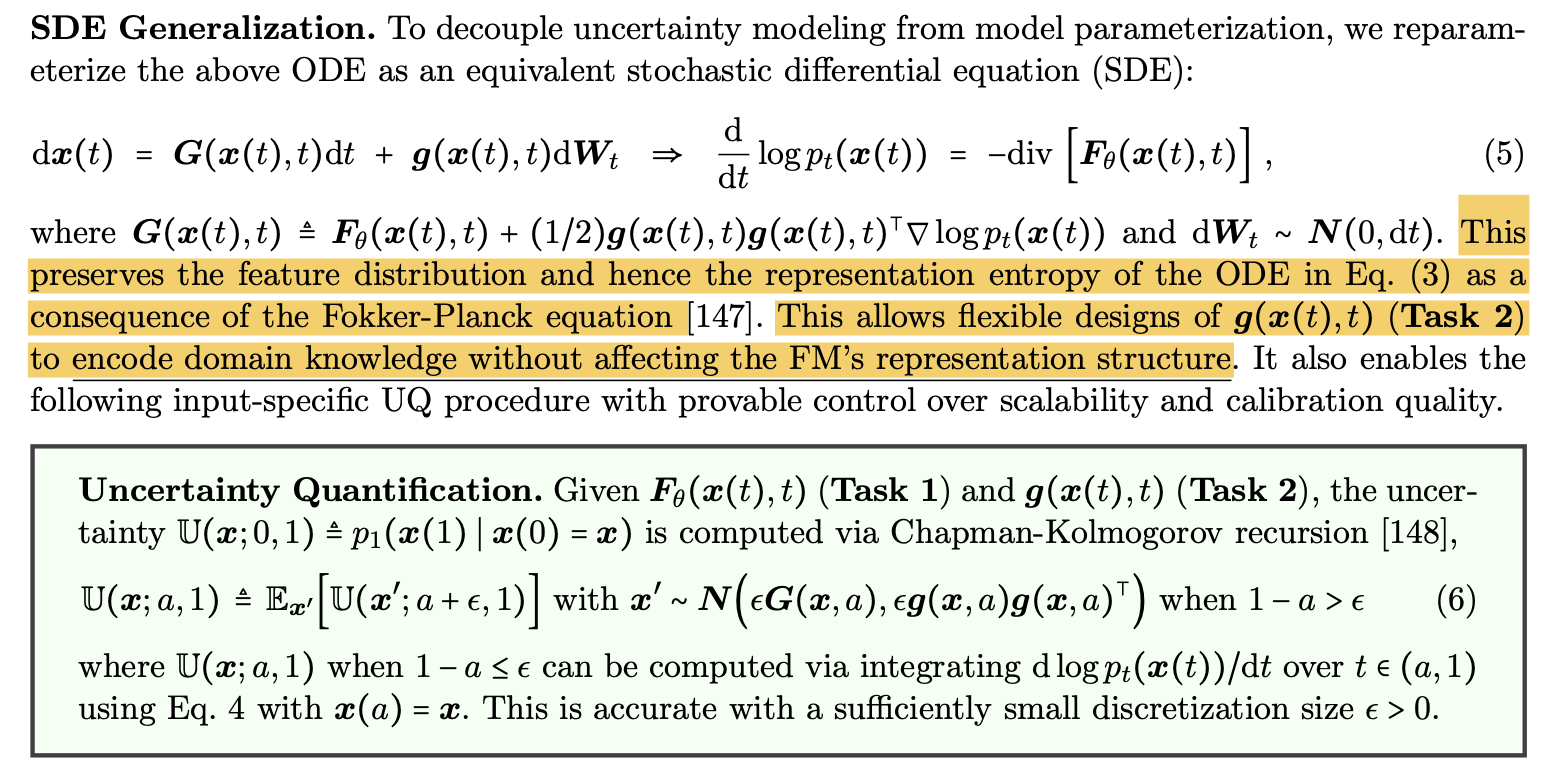
\includegraphics[width=0.94\linewidth,height=0.74\textheight,keepaspectratio]{user_eq5_eq6.png}
  \source{Screenshot from the proposal, Section 3.2 (highlights added).}
\end{frame}

% ------------------------------------------------------------
\begin{frame}{What Fokker--Planck actually guarantees}
  \begin{columns}[T,onlytextwidth]
    \column{0.48\textwidth}
    \begin{block}{Guaranteed}
      If $\x(0)\sim p_0$, the SDE and the ODE share the \textbf{population marginals} $p_t$ for every $t$, hence the same marginal entropy $H(\x(t))$.
    \end{block}
    \column{0.48\textwidth}
    \begin{alertblock}{Not guaranteed}
      The \textbf{conditional law} $p(\x(1)\mid\x(0)=\x)$ --- exactly the object $\U(\x;0,1)$ that Eq.~(6) computes --- can be anything.
    \end{alertblock}
  \end{columns}
  \smallskip
  \textbf{Two corrections to Eq.~(5)}
  \begin{itemize}
    \item With a \emph{state-dependent} scaffold (Task 2), the drift that keeps $p_t$ is
      \[
        \G=\Ft+\tfrac12\,\D\,\nabla\log p_t+\tfrac12\,\nabla\!\cdot\D,\qquad \D=\g\g^\top .
      \]
    \item $\frac{d}{dt}\log p_t(\x(t))=-\operatorname{div}\Ft$ holds along \textbf{ODE characteristics}, not along SDE sample paths (Itô terms appear).
  \end{itemize}
\end{frame}

% ------------------------------------------------------------
\begin{frame}{Counterexample: same marginal, the output forgets the input}
  \small
  $\Ft=0$, \ $p_0=\mathcal N(0,1)$, \ $\g=\sigma$ \ $\Rightarrow$ \ Eq.~(5) gives
  $d\x=-\tfrac{\sigma^2}{2}\x\,dt+\sigma\,d\bm W_t$ (Ornstein--Uhlenbeck), with
  \[
    p_t=\mathcal N(0,1)\ \ \forall t,\qquad
    \E[\x(1)\mid\x_0]=e^{-\sigma^2/2}\x_0,\qquad
    \Var[\x(1)\mid\x_0]=1-e^{-\sigma^2}.
  \]
  \vspace{-0.6em}
  \centering
  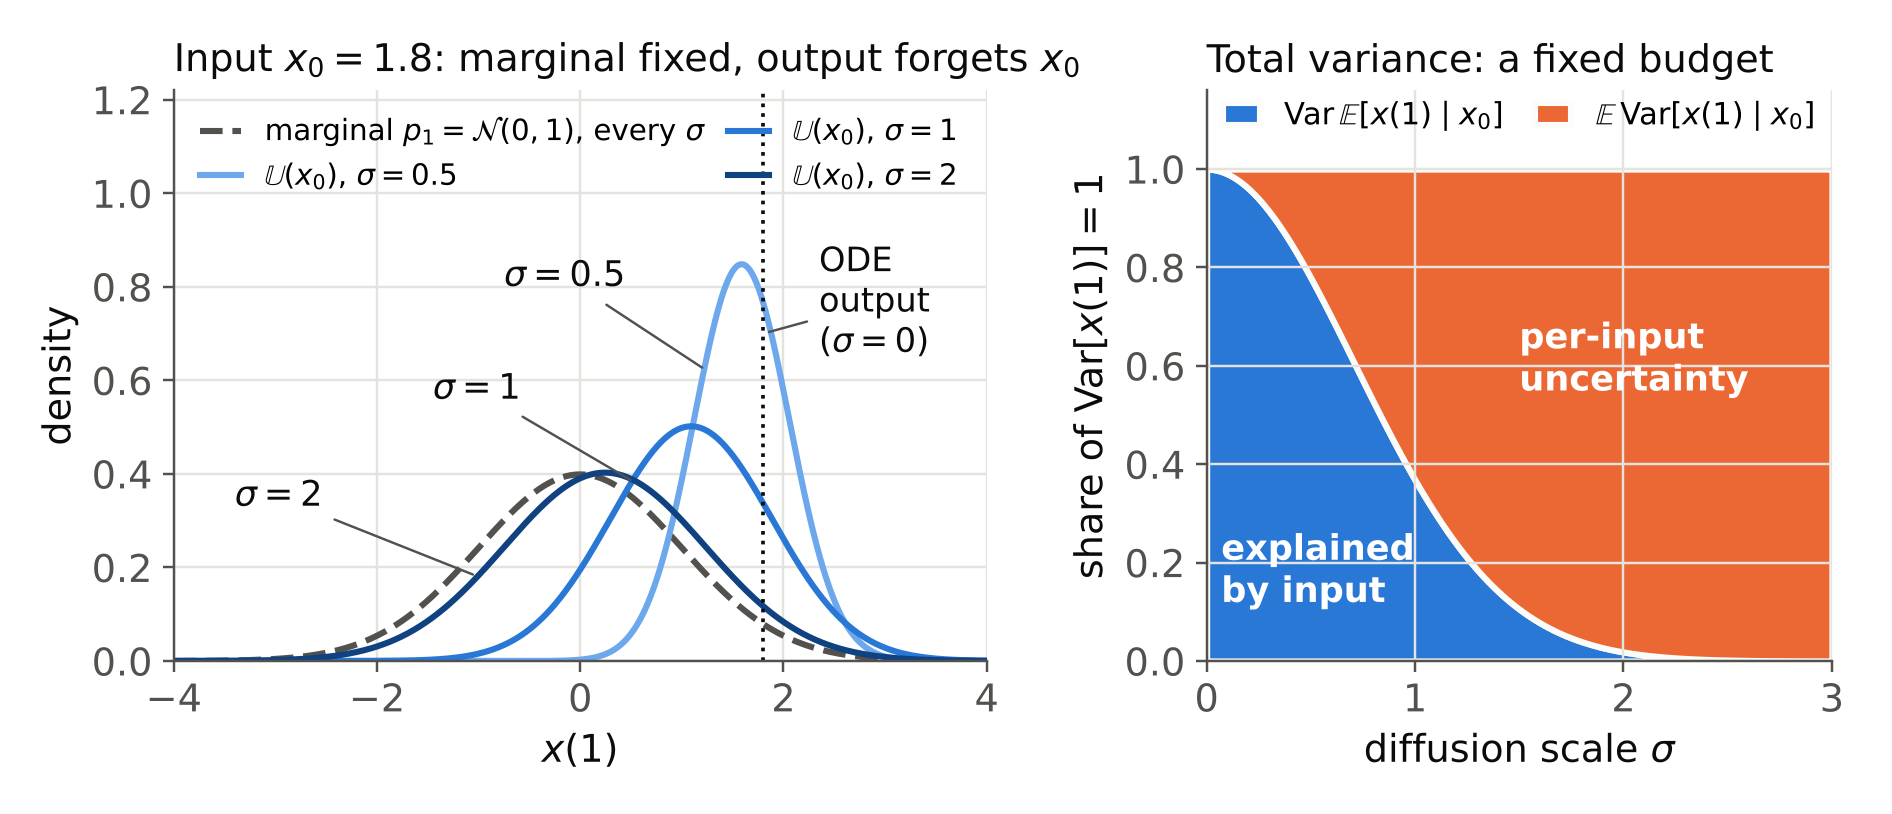
\includegraphics[width=0.92\linewidth,height=0.62\textheight,keepaspectratio]{fig_ou_same_marginal.png}
\end{frame}

% ------------------------------------------------------------
\begin{frame}{Why $\g$ is not a free design choice}
  \small
  \textbf{A fixed budget.} Because $p_1$ is fixed,
  \[
    \underbrace{\Var[\x(1)]}_{\text{fixed}}
    =\underbrace{\E\,\Var[\x(1)\mid\x_0]}_{\text{uncertainty from }\g}
    +\underbrace{\Var\,\E[\x(1)\mid\x_0]}_{\text{explained by the input}},
    \qquad
    \underbrace{H(\x(1))}_{\text{fixed}} = H(\x(1)\mid\x_0)+I(\x_0;\x(1)).
  \]
  Every unit of uncertainty added by $\g$ is paid for with \alert{shrinkage} of the conditional means and \alert{lost mutual information} with the input.
  \smallskip
  \begin{itemize}
    \item \textbf{No link to Eq.~(1).} $\U$ is set entirely by $\g$; the Bayesian pushforward of $p(\theta\mid\mathcal D)$ usually \emph{widens} the marginal, so it lies outside the same-marginal family.
    \item \textbf{Hidden requirement.} $\G$ needs the population score $\nabla\log p_t$, i.e.\ a score or density model of the input-embedding distribution $p_0$.
    \item \textbf{Unspecified coupling.} Independent noise per input gives no epistemic correlation between $f(\x_a)$ and $f(\x_b)$; a shared $\bm W$ gives some. ECE/NLL cannot tell them apart.
  \end{itemize}
\end{frame}

% ------------------------------------------------------------
\begin{frame}{Eq.~(6): the recursion as written}
  \begin{itemize}
    \item \textbf{Mean.} The Euler kernel is $\x'\sim\mathcal N\big(\x+\epsilon\G(\x,a),\ \epsilon\,\D\big)$: the term $\x$ is missing.
    \item \textbf{Terminal step.} The backward recursion needs $\U(\x;1,1)=\delta(\x(1)-\x)$. Eq.~(4) is the \emph{marginal} change-of-variables along the ODE, not a conditional density. The natural last step is the kernel itself:
      \[
        \U(\x;1-\epsilon,1)=\mathcal N\big(\x(1);\ \x+\epsilon\G,\ \epsilon\D\big),
      \]
      so $\U(\x;0,1)$ is a Gaussian mixture with $N^{1/\epsilon}$ components.
    \item \textbf{Cost and accuracy.}
      \begin{itemize}
        \item The $O(e^{-N})$ rate is per dimension, for analytic integrands; a tensor grid in $d$ dimensions needs $N^{d}$ nodes ($d\approx 384$--$768$).
        \item Errors accumulate: total $O(\delta/\epsilon+\epsilon)$, not $O(\delta)$.
        \item $O(\delta)$ is numerical error w.r.t.\ the model's own $\U$, \alert{not calibration error} w.r.t.\ the labels.
      \end{itemize}
  \end{itemize}
\end{frame}

% ------------------------------------------------------------
\section{Claim 4: the reference scaffold}

\begin{frame}{The text under review: Eq.~(8)}
  \centering
  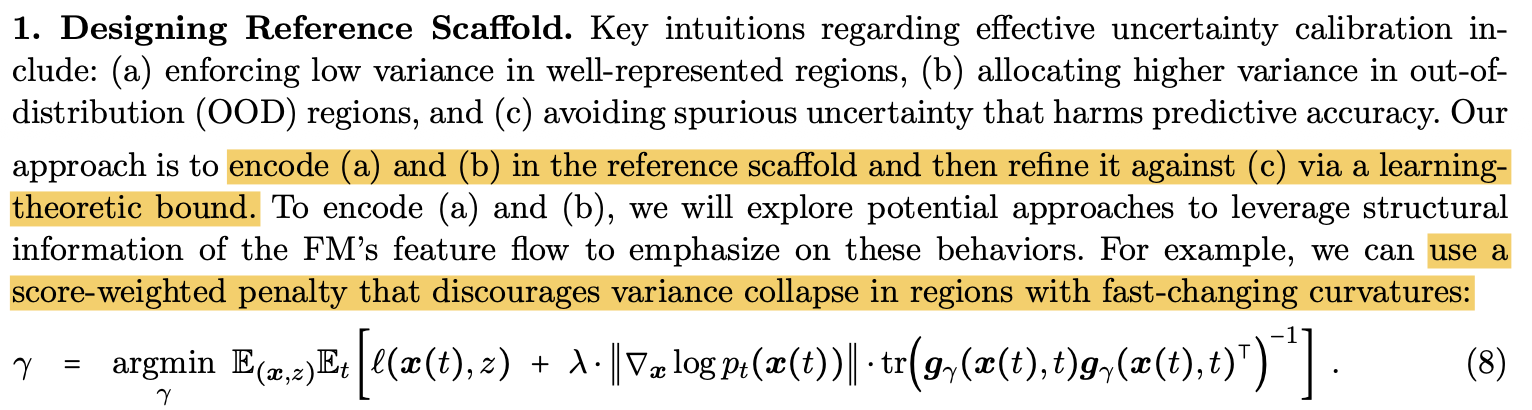
\includegraphics[width=0.94\linewidth]{user_eq8_clean.png}
  \source{Screenshot from the proposal, Section 3.2, Task 2 (highlights added; blank band removed).}
\end{frame}

% ------------------------------------------------------------
\begin{frame}{A score is not a curvature}
  \begin{columns}[c,onlytextwidth]
    \column{0.60\textwidth}
    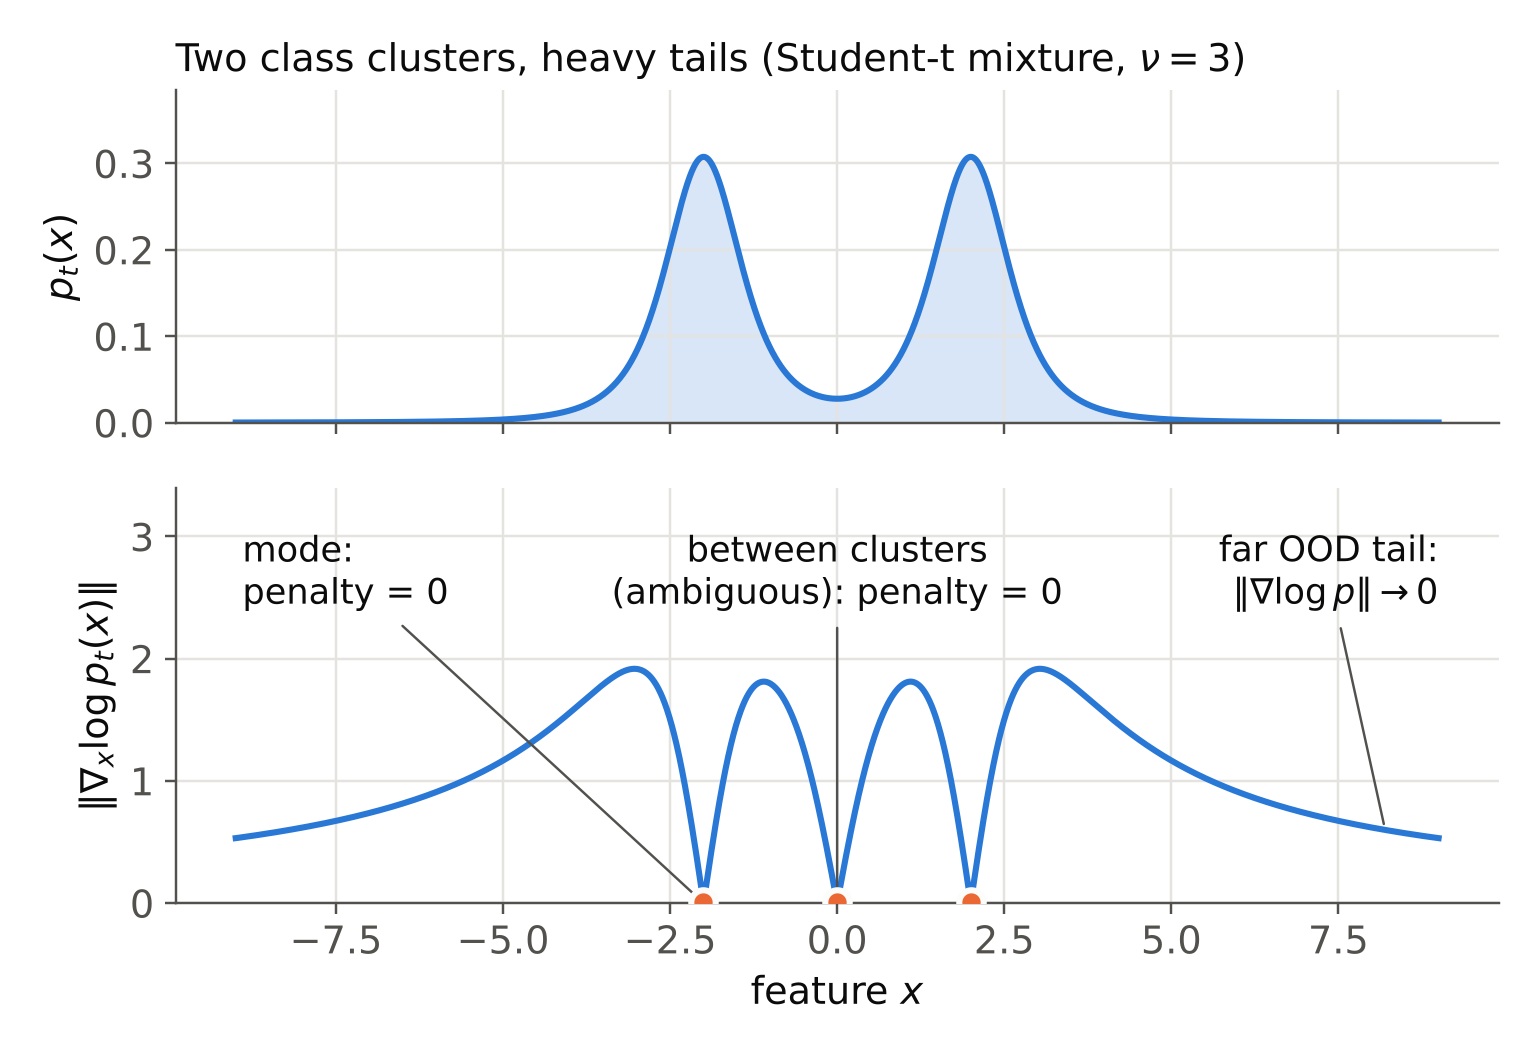
\includegraphics[width=\linewidth,height=0.8\textheight,keepaspectratio]{fig_score_penalty.png}
    \column{0.37\textwidth}
    \footnotesize
    $\|\nabla_{\x}\log p_t\|$ is first order; a curvature would be the Hessian. The penalty vanishes:
    \begin{itemize}
      \item at every \textbf{mode};
      \item \textbf{between clusters}, where ambiguous inputs sit;
      \item in \textbf{heavy tails}, far OOD.
    \end{itemize}
    The score is learned from training features, so it is \alert{least reliable OOD}, exactly where it is used.
  \end{columns}
\end{frame}

% ------------------------------------------------------------
\begin{frame}{What Eq.~(8) actually optimizes}
  Let $T=\operatorname{tr}(\g\g^\top)$ and approximate the loss increase as $c\,T$, with $c$ the loss curvature in feature space:
  \[
    \min_T\ c\,T+\lambda\,\frac{\|\nabla\log p_t\|}{T}
    \quad\Rightarrow\quad
    T^\star\approx\sqrt{\lambda\,\|\nabla\log p_t\|\,/\,c}.
  \]
  \vspace{-0.5em}
  \begin{itemize}
    \item \textbf{(b) is inverted near decision boundaries.} The CE Hessian in logits, $\operatorname{diag}(p)-pp^\top$, is largest when $p$ is near uniform, so $c$ is largest and $T^\star$ smallest for ambiguous inputs.
    \item \textbf{(a) is not encoded.} Near the modes the penalty is zero and variance is set by the loss alone.
    \item \textbf{$\ell(\x(t),z)$ at intermediate $t$} needs a prediction head at every $t$; the proposal only defines $h(\x(1))$.
  \end{itemize}
\end{frame}

% ------------------------------------------------------------
\begin{frame}{The refinement bound (Eq.~9) cannot refine}
  \small
  \[
    \E\,\ell_\phi \;\le\; \underbrace{\tfrac1n\textstyle\sum_i \ell_\gamma(\x_i,z_i)}_{\text{independent of }\phi}
    \;+\;\min_\varphi\Big\{\tau_\varphi\,\E_{\x}\,W_\varphi\big(p_\phi(\cdot\mid\x),p_\gamma(\cdot\mid\x)\big)\Big\}
    \;+\;\varepsilon_{\mathcal D}(n,\delta,\gamma)
  \]
  \begin{itemize}
    \item The only $\phi$-dependent term is the distance to $\gamma$, so minimizing the bound returns \alert{$\phi=\gamma$}: nothing is refined against (c).
    \item \textbf{Fix:} a PAC-Bayes-style bound with an empirical $\tfrac1n\sum_i\ell_\phi$ term plus a deviation penalty to $\gamma$, with $\gamma$ fitted on held-out data (or a uniform/stability argument over the scaffold class).
    \item Kantorovich--Rubinstein needs $\ell_\phi=\E_{u\sim p_\phi}\ell(u,z)$ (a per-sample loss). The NLL of the averaged prediction, $-\log\E_u\,p(z\mid u)$, is not of this form.
    \item Taking $\min_\varphi$ is harmless at population level; data dependence enters only if $\E_{\x}W_\varphi$ is estimated on the training sample.
  \end{itemize}
\end{frame}

% ------------------------------------------------------------
\section{Pilot experiments}

\begin{frame}{Pilot setup}
  \small
  \begin{itemize}
    \item \textbf{Data.} sklearn digits ($8\times8$). Classes 0--8 are ID; OOD = held-out digit 9, $90^\circ$ rotations, uniform noise. A \emph{shift} set (test digits + pixel noise, $\sigma=0.3$) keeps labels.
    \item \textbf{FM.} 4-block pre-LN ViT, $d=64$, dropout $0.1$, trained from scratch ($\approx98\%$ ID accuracy). 5 random splits; mean $\pm$ sd.
    \item \textbf{References.} MC dropout and a 5-member deep ensemble (member 0 = the FM).
    \item \textbf{Same-marginal SDE family without learning $\Ft$ or a score.} Lie--Trotter splitting: run the FM block exactly ($p_l\mapsto p_{l+1}$), then $K$ MALA steps targeting $p_{l+1}$, with the score of a class-conditional GMM fitted to training features. MALA keeps the (GMM) marginal exactly.
    \item \textbf{Baselines.} Temperature scaling (TS), MC dropout, ensemble, and the GMM's own Mahalanobis OOD score (free once the GMM exists).
  \end{itemize}
  \source{Code: \texttt{uq/experiments/} (CPU only). Reproduce with \texttt{bash run\_all.sh}.}
\end{frame}

% ------------------------------------------------------------
\begin{frame}{Exp.~0: is the reference inside the same-marginal family?}
  \centering
  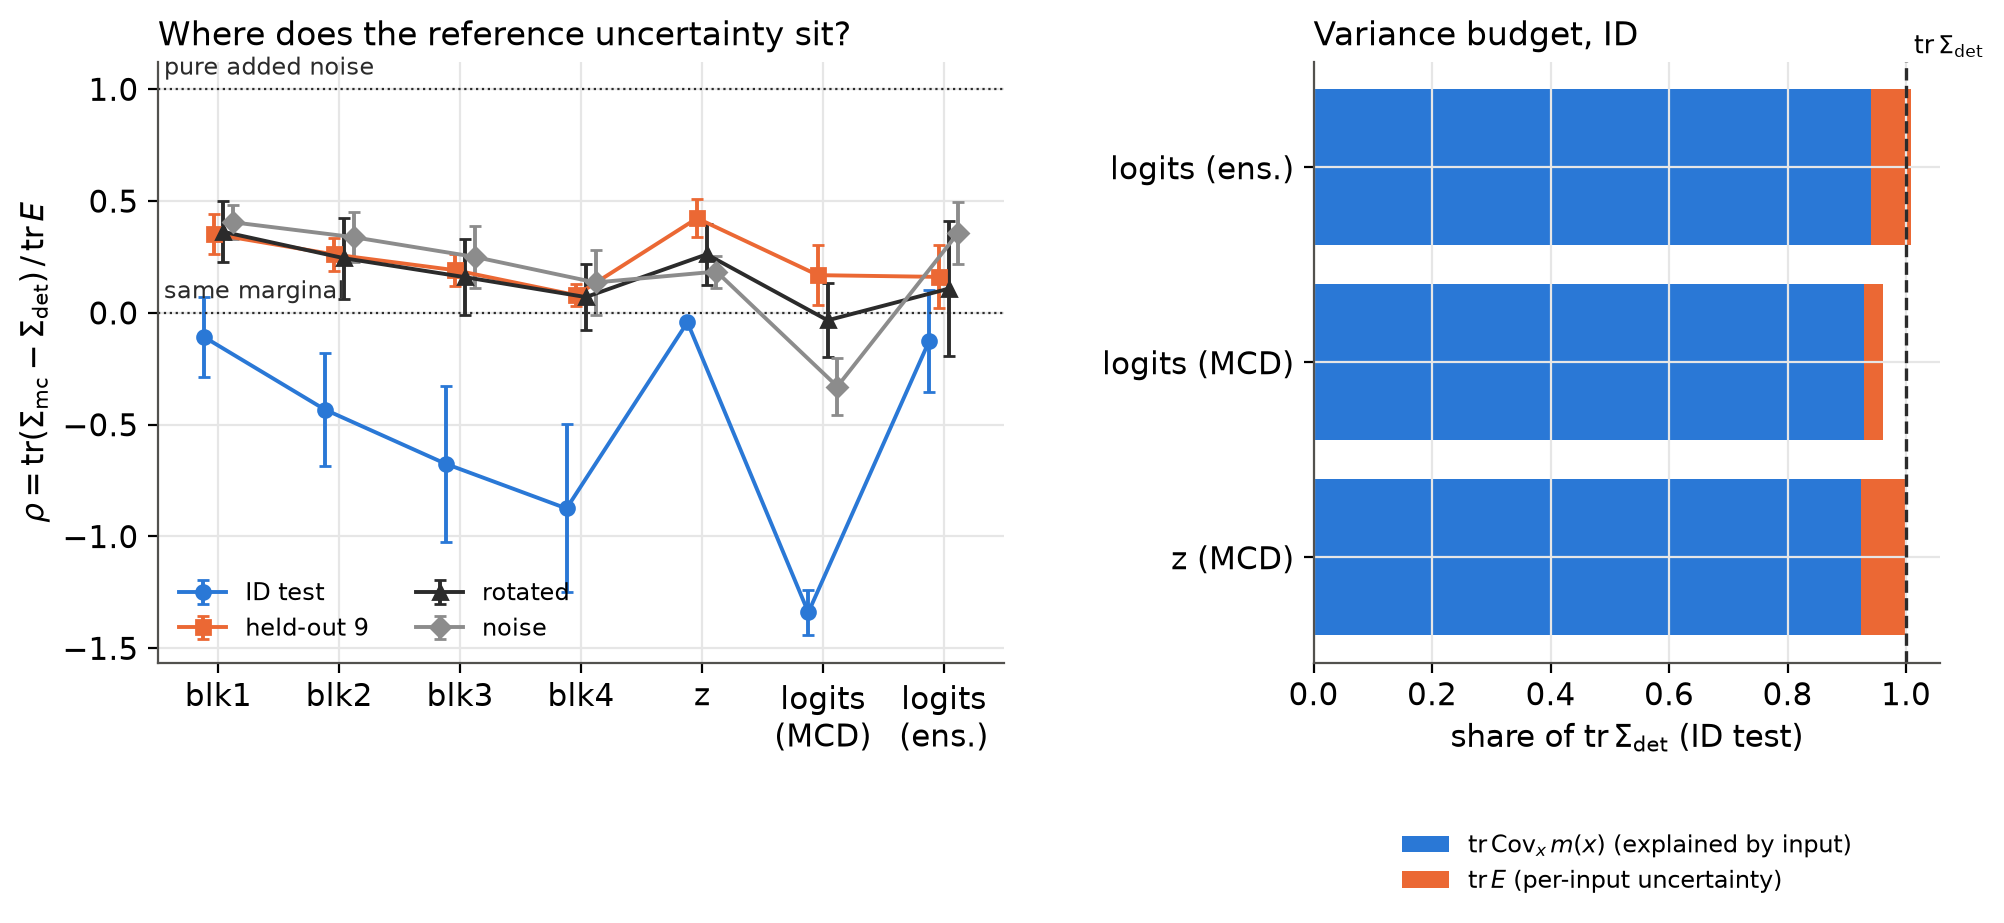
\includegraphics[width=\linewidth,height=0.6\textheight,keepaspectratio]{fig_exp0_rho.png}
  \footnotesize
  \begin{itemize}
    \item \textbf{ID, final representation $z$:} $\rho=-0.04\pm0.004$. MC dropout's population variance \emph{matches} the deterministic one at trace level; its per-input variance (7.6\% of the budget) is paid for by shrinking the means.
    \item \textbf{ID, logits:} $\rho=-1.34$, so dropout \emph{removes} variance. \textbf{OOD:} $\rho\approx0.2$--$0.4$, so it adds variance, which the family is free to do off $p_0$.
  \end{itemize}
\end{frame}

% ------------------------------------------------------------
\begin{frame}{Quick test: the $\tfrac12\nabla\!\cdot\D$ term is needed}
  \begin{columns}[c,onlytextwidth]
    \column{0.58\textwidth}
    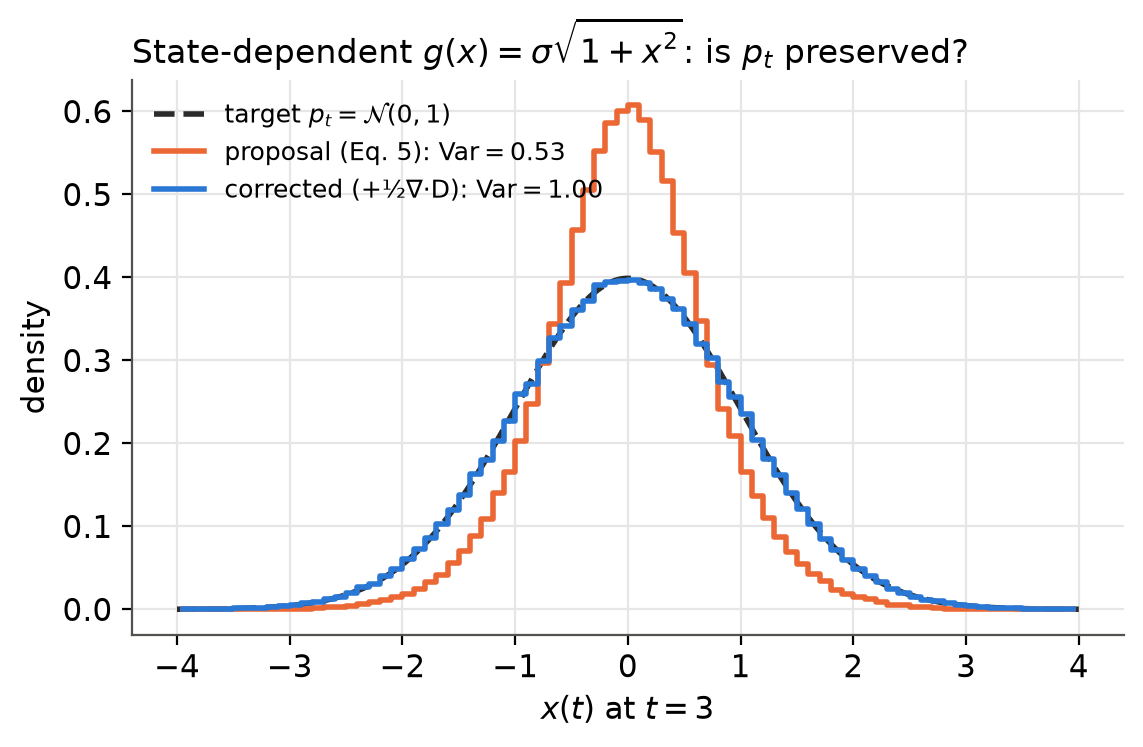
\includegraphics[width=\linewidth]{fig_q2_drift_correction.png}
    \column{0.39\textwidth}
    \small
    $\Ft=0$, $p_0=\mathcal N(0,1)$, $\g(x)=1.5\sqrt{1+x^2}$.
    \begin{itemize}
      \item Drift as in Eq.~(5): $p_t$ \alert{shrinks} to Var $0.53$ (analytic stationary value $0.525$).
      \item With $+\tfrac12\nabla\!\cdot\D$: Var $1.00$, KS distance $0.001$.
    \end{itemize}
  \end{columns}
\end{frame}

% ------------------------------------------------------------
\begin{frame}{Quick test: Eq.~(6) tree vs.\ Monte Carlo paths}
  \centering
  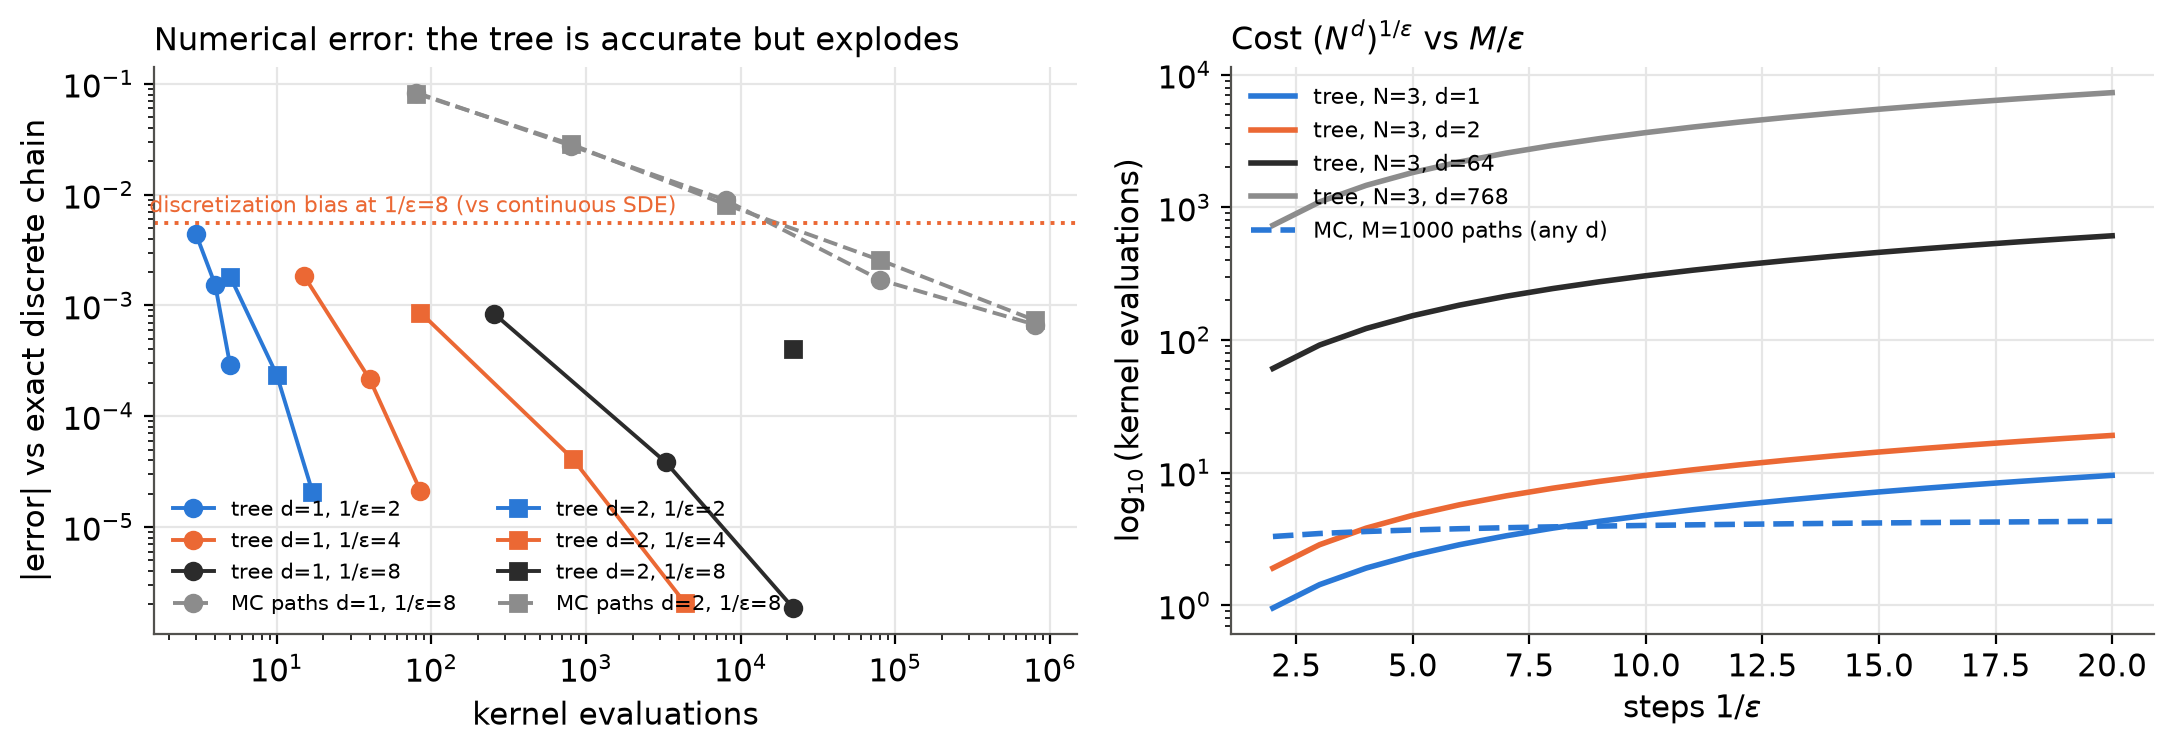
\includegraphics[width=\linewidth,height=0.62\textheight,keepaspectratio]{fig_q3_eq6_cost.png}
  \footnotesize
  \begin{itemize}
    \item In $d\le2$ the Gauss--Hermite tree is very accurate ($10^{-6}$ against the discrete chain), but its cost is $(N^d)^{1/\epsilon}$: about $10^{7300}$ evaluations for $d=768$.
    \item Error against the \emph{continuous} SDE is set by discretization ($0.0055$ at $1/\epsilon=8$), which neither method removes. Monte Carlo costs $M/\epsilon$ in any dimension.
  \end{itemize}
\end{frame}

% ------------------------------------------------------------
\begin{frame}{Quick test: where does Eq.~(8) put the variance?}
  \centering
  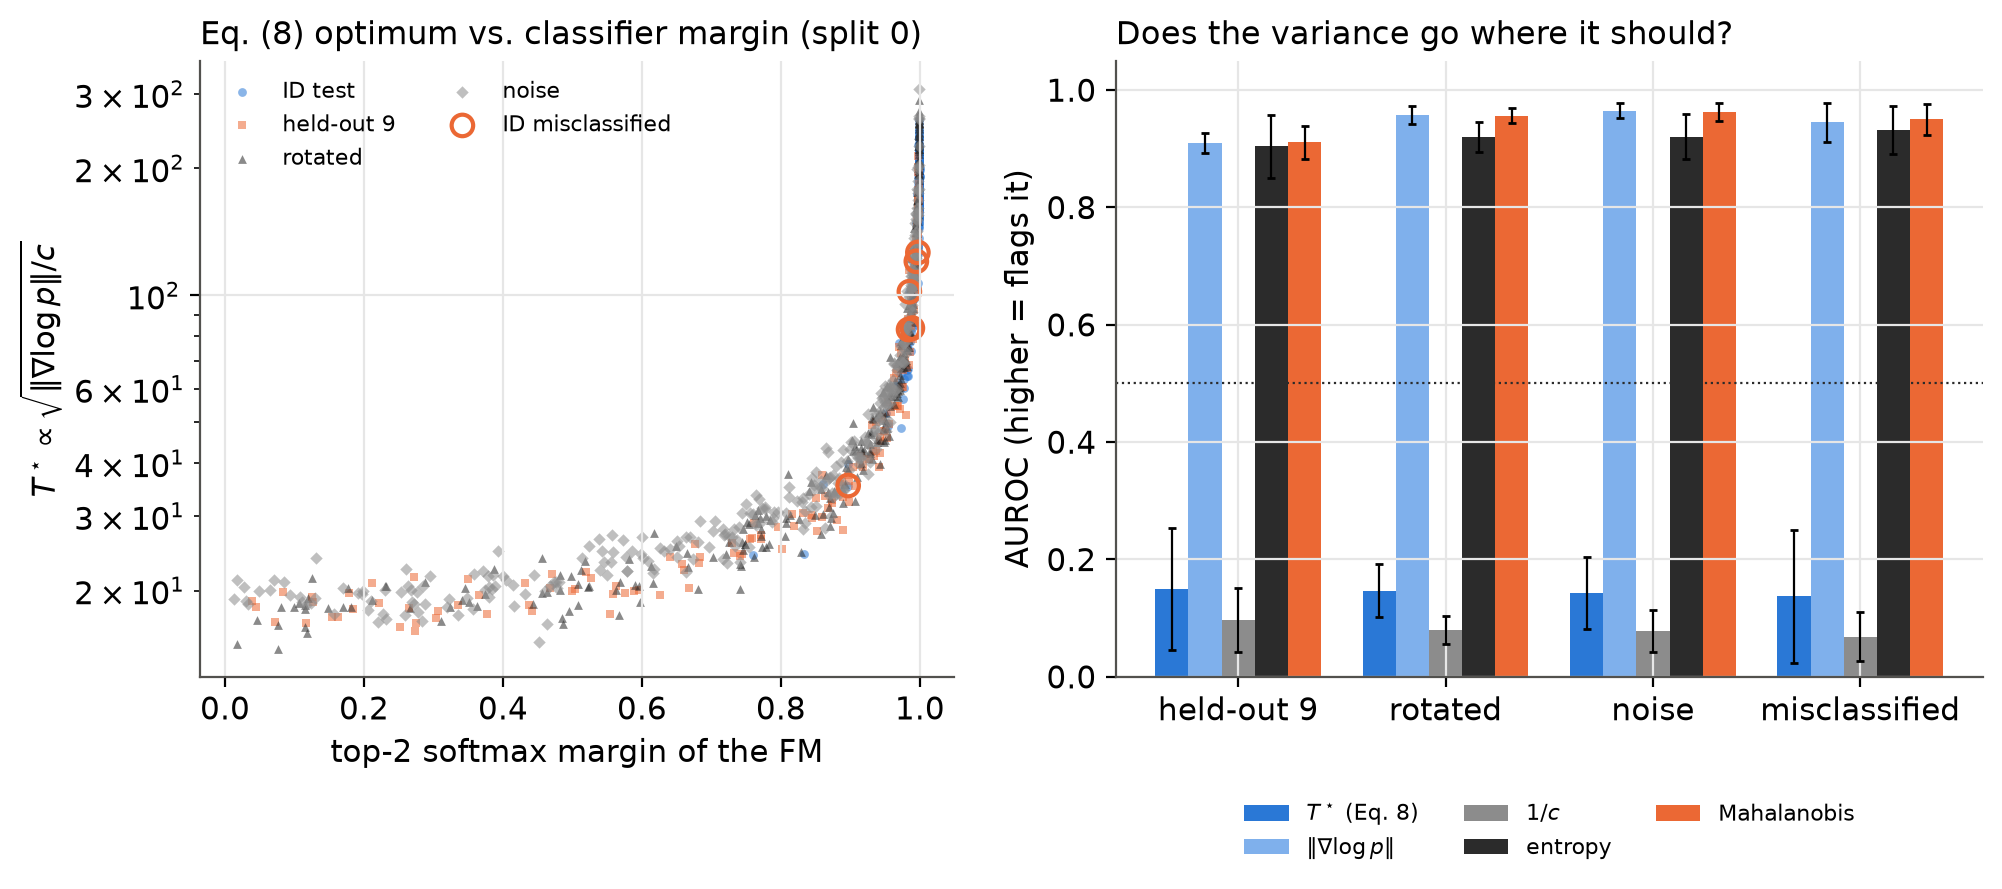
\includegraphics[width=\linewidth,height=0.62\textheight,keepaspectratio]{fig_q4_eq8_penalty.png}
  \footnotesize
  \begin{itemize}
    \item $T^\star$ flags OOD and misclassified inputs with AUROC $0.14$--$0.15$, \alert{well below chance}: the loss curvature $c$ is largest on ambiguous inputs and wins.
    \item With a Gaussian score model, $\|\nabla\log p\|$ alone is a good OOD score ($0.91$--$0.97$), essentially Mahalanobis.
  \end{itemize}
\end{frame}

% ------------------------------------------------------------
\begin{frame}{Exp.~1: sweeping the same-marginal SDE family}
  \centering
  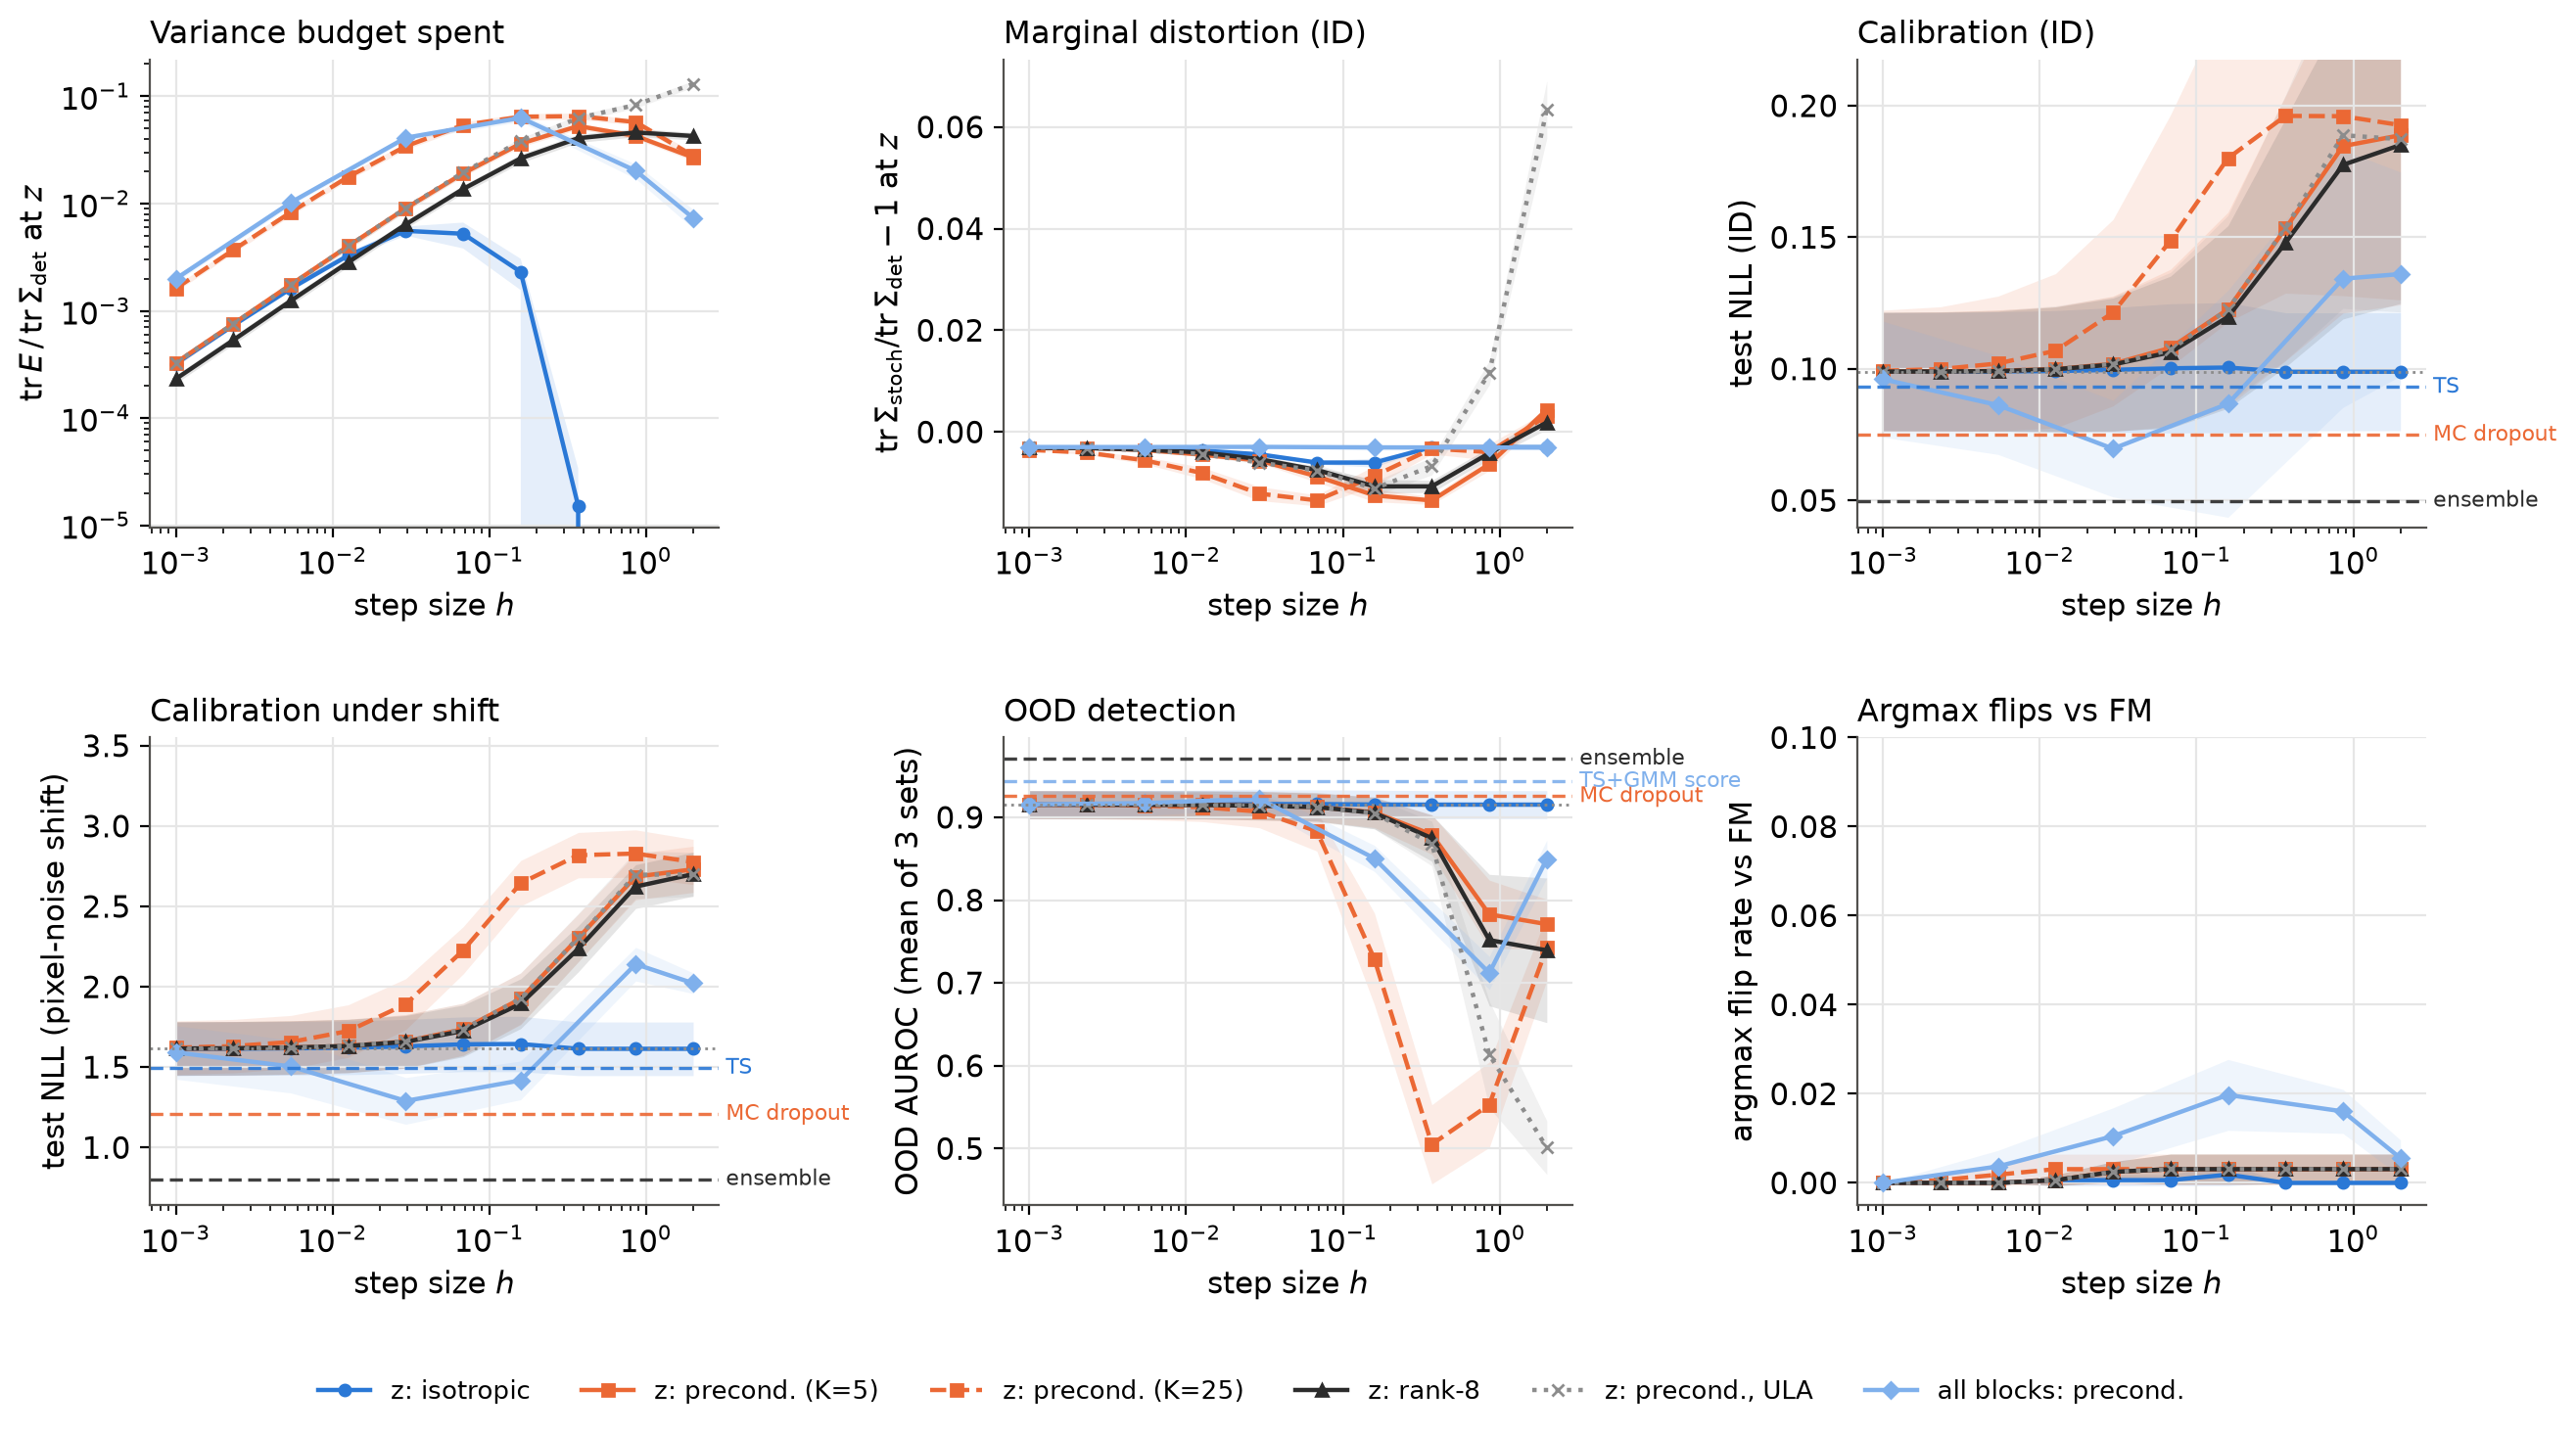
\includegraphics[width=\linewidth,height=0.84\textheight,keepaspectratio]{fig_exp1_sweep.png}
  \source{The isotropic curve stays flat at large $h$ because MALA rejects every proposal there, not because it is stable. $D$ uses the GMM's within-class covariance; with the population covariance, MALA rejects everything and ULA diverges.}
\end{frame}

% ------------------------------------------------------------
\begin{frame}{Exp.~1: the decisive question}
  \footnotesize
  \centering
  \begin{tabular}{@{}lcccccc@{}}
    \toprule
    Method & Acc & NLL & ECE\,\% & Shift NLL & Shift ECE\,\% & OOD AUROC\\
    \midrule
    FM & .978 & .099 & 1.8 & 1.61 & 23.7 & .915\\
    Temperature scaling & .978 & .093 & 1.7 & 1.49 & 22.6 & .916\\
    MC dropout & .979 & .075 & 1.5 & 1.21 & 14.8 & .925\\
    Deep ensemble (5) & \textbf{.990} & \textbf{.050} & 1.5 & \textbf{0.80} & \textbf{6.4} & \textbf{.971}\\
    TS + GMM Mahalanobis score & .978 & .093 & 1.7 & 1.49 & 22.6 & .943\\
    \midrule
    SDE, Langevin on $z$ only & .978 & .100 & 1.9 & 1.63 & 24.5 & .915\\
    SDE, Langevin after every block & .984 & .080 & 1.5 & 1.31 & 17.6 & .905\\
    \bottomrule
  \end{tabular}
  \par\smallskip
  \raggedright
  SDE rows use the configuration with the best \emph{validation} NLL per split. Mean over 5 splits.
  \begin{itemize}
    \item \alert{No configuration} beats TS on NLL+ECE \emph{and} MC dropout on OOD AUROC, even when picked on test, with or without TS on top.
    \item Langevin after every block helps calibration over TS, but trails MC dropout and \emph{lowers} OOD AUROC.
    \item Langevin on $z$ only: low-margin inputs become \emph{more} confident ($+2.7$\,pp): the mixture score pulls them toward a class mode.
  \end{itemize}
\end{frame}

% ------------------------------------------------------------
\begin{frame}{What the pilot says}
  \small
  \begin{itemize}
    \item \textbf{The tension is real but not where expected.} In-distribution, the MC-dropout reference sits at $\rho\approx0$ at $z$; the problem is not lack of variance budget but \emph{where} the family spends it.
    \item \textbf{The score drift shrinks toward modes.} It sharpens ambiguous inputs, and OOD detection gets worse as $h$ grows (consistent with OOD inputs being pulled toward the data).
    \item \textbf{Eq.~(8) is inverted in practice}, not only in theory.
    \item \textbf{H0 holds on this pilot:} the uncertainty mechanism does not beat simple baselines. The free GMM Mahalanobis score is the strongest single-model OOD detector here.
  \end{itemize}
  \smallskip
  {\footnotesize Caveats: easy pilot (about 7 ID errors per split, so ID ECE is noisy); GMM stand-in for the score; $\rho$ only compares traces. The ImageNet ablation ladder (Exp.~2) is next.}
\end{frame}

% ------------------------------------------------------------
\section{What to do next}

\begin{frame}{Suggested fixes and quick tests}
  \small
  \begin{tabular}{@{}>{\raggedright\arraybackslash}p{0.25\linewidth}>{\raggedright\arraybackslash}p{0.35\linewidth}>{\raggedright\arraybackslash}p{0.34\linewidth}@{}}
    \toprule
    \textbf{Issue} & \textbf{Fix} & \textbf{Quick test}\\
    \midrule
    Marginal $\neq$ conditional & State the target: same marginal, or Bayesian pushforward & Ratio $\operatorname{tr}(\Sigma_{\mathrm{MC}}-\Sigma_{\mathrm{det}})/\operatorname{tr}\E\,\mathrm{Cov}$ vs.\ MC dropout\\
    State-dependent $\g$ & Add $\tfrac12\nabla\!\cdot(\g\g^\top)$ to the drift & Check $p_1$ is unchanged numerically\\
    Eq.~(6) & Gaussian terminal kernel; Monte Carlo or moment matching & Error vs.\ cost against MC paths\\
    Eq.~(8) & Distance-aware term; not the raw score & $T^\star$ at modes, saddle, far OOD\\
    Eq.~(9) & Empirical $\ell_\phi$ term; held-out $\gamma$ & Does the minimizer move away from $\gamma$?\\
    \bottomrule
  \end{tabular}
\end{frame}

% ------------------------------------------------------------
\begin{frame}{Summary}
  \small
  \begin{itemize}
    \item Preserving the \textbf{marginal} $p_t$ does not preserve the \textbf{per-input representation}: with $p_1$ fixed, every bit of uncertainty from $\g$ is paid for in shrinkage and lost mutual information.
    \item Hence $\g$ is a trade-off knob, not a free design choice, and $\U$ is not tied to the posterior pushforward of Eq.~(1).
    \item Eq.~(6) needs a correct mean, a correct terminal step, and an honest cost model in $d$ dimensions.
    \item The score-weighted penalty is zero where uncertainty matters most (modes, between clusters, heavy tails), and Eq.~(9) is minimized at $\phi=\gamma$.
  \end{itemize}
  \smallskip
  \begin{block}{Open question for the group}
    Which object should Thrust 1 preserve: the marginal $p_t$, the conditional $p(\x(1)\mid\x)$, or the function-level joint $p(f(\x_a),f(\x_b)\mid\mathcal D)$?
  \end{block}
\end{frame}

% ============================================================
%  TEMPLATE: a slide with your own image.
%  Upload your image to figures/, uncomment, and edit the name.
% ------------------------------------------------------------
% \begin{frame}{Title of your slide}
%   \centering
%   \includegraphics[width=0.9\linewidth]{your_image.png}
%   \source{Caption or source of the image.}
% \end{frame}
%
%  Two images side by side:
% \begin{frame}{Two images}
%   \begin{columns}[c,onlytextwidth]
%     \column{0.49\textwidth}\includegraphics[width=\linewidth]{image_left.png}
%     \column{0.49\textwidth}\includegraphics[width=\linewidth]{image_right.png}
%   \end{columns}
% \end{frame}
% ============================================================

\end{document}
